\section{Beam Search to Support Patch Validation}

\begin{figure}[t]
	\centering
	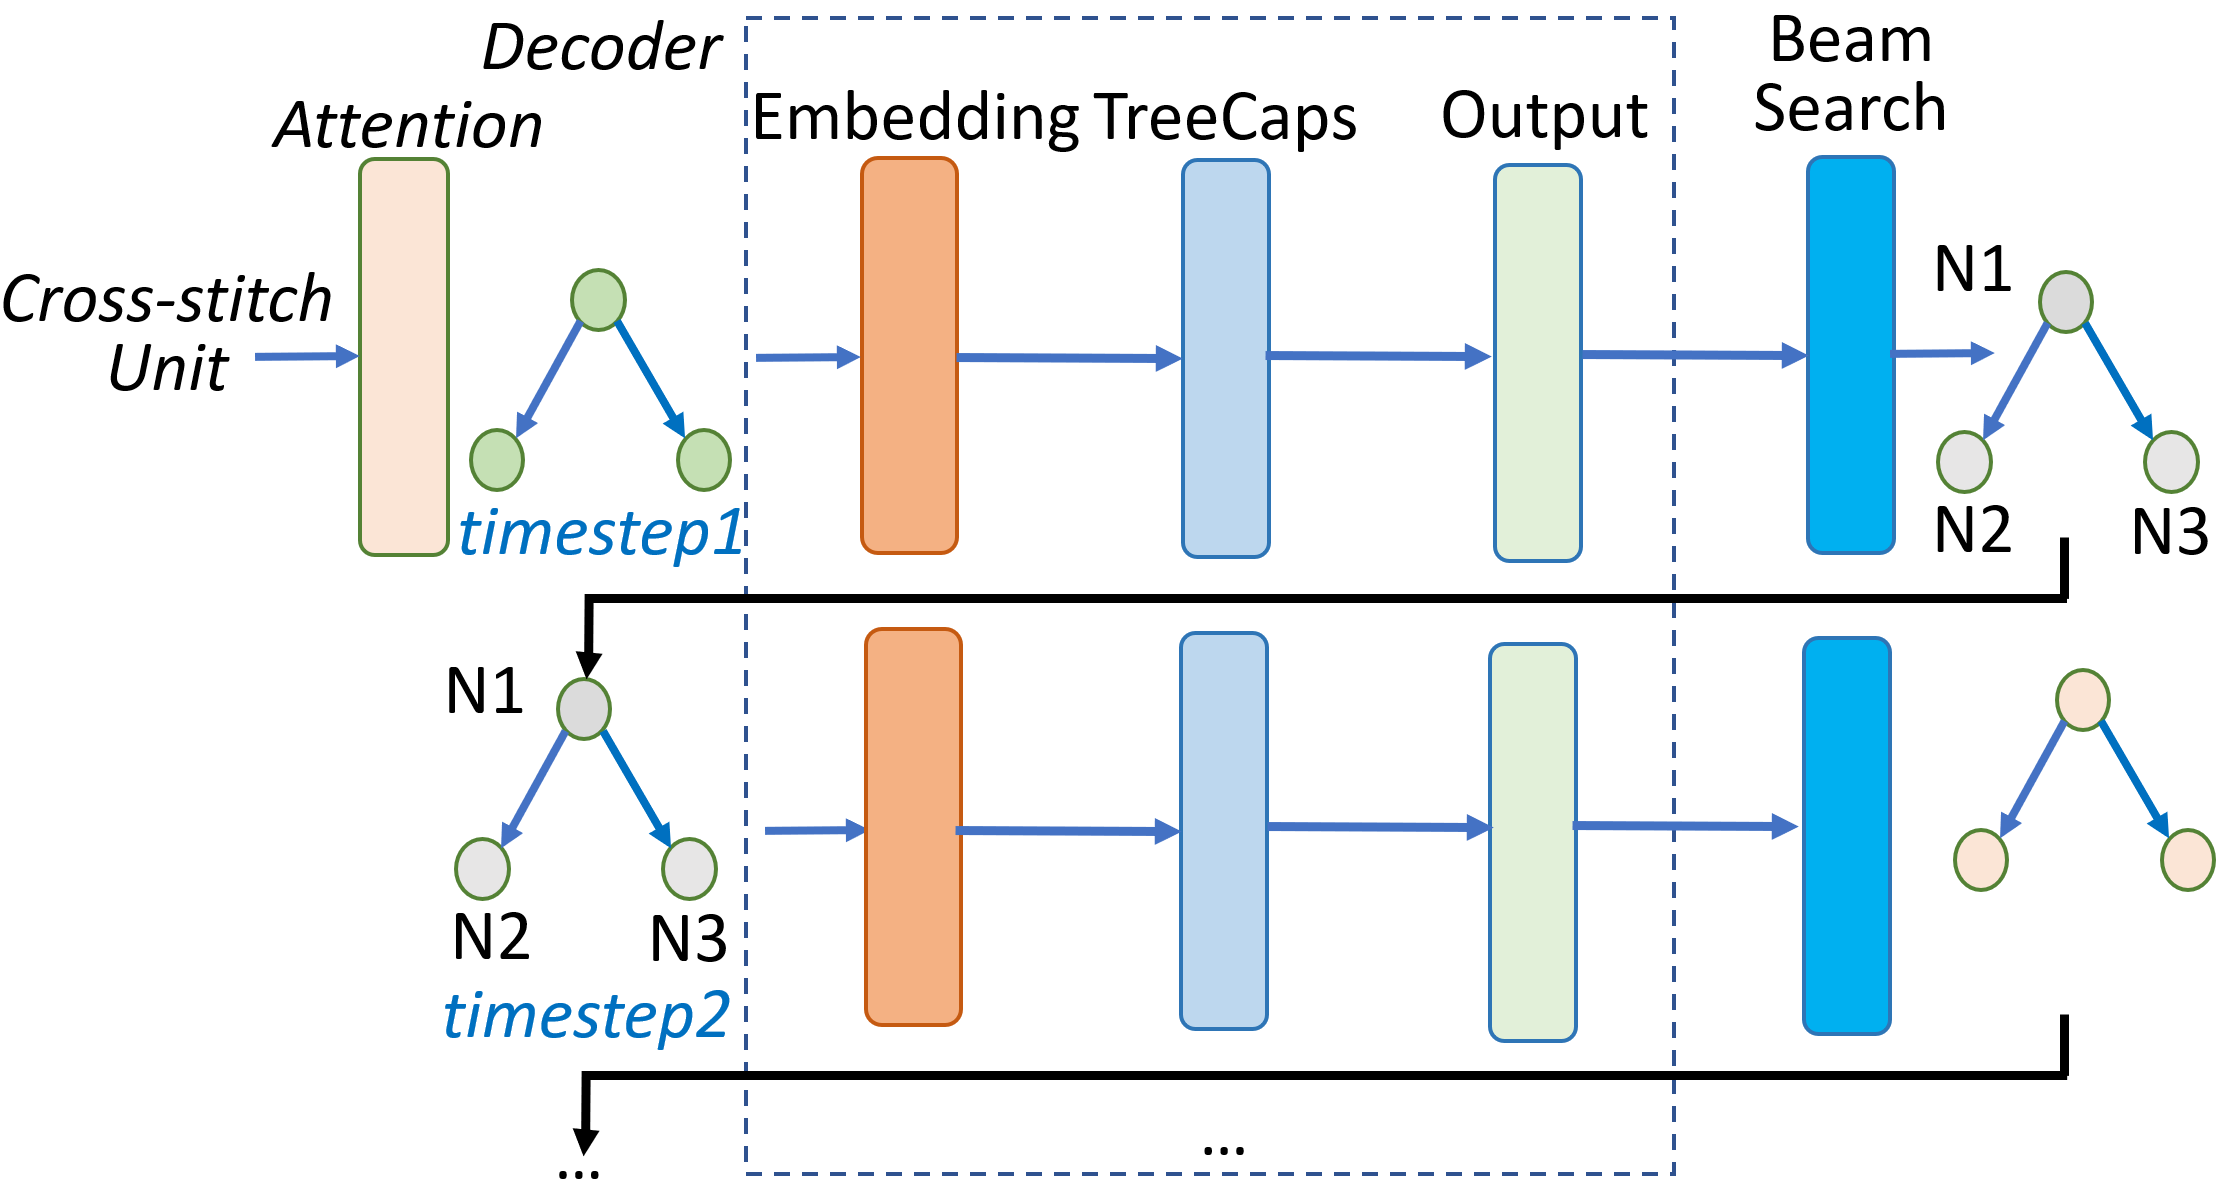
\includegraphics[width=3.2in]{graphs/beam-search.png}
	\caption{Tree-Structured Beam Search for Patch Generation}
	\label{beam}
\end{figure}

%\begin{algorithm}[t]
	\caption{Tree-structured Beam Search}
	\label{algo}
	\scriptsize
	\begin{algorithmic}[1]
		\Function {TreeStructuredBeamSearch}{$NodeList, Dictionary, BeamSize$}
		\State $HeightList = GetNodeHeight(NodeList)$ 
		\State $ReorderedNodeList = ReorderList(NodeList, HeightList)$ % Based on node height in the tree to rerank all nodes
		\If {$N_i,N_j \in ReorderedNodeList$ $\textbf{\&}$ $HaveSameParent(N_i, N_j)$}
			\State $GroupedNodeList = GroupStatement(ReorderedNodeList, N_i, N_j)$ %If two nodes have the same parent node, we group them as one
		\EndIf
		\State $Result = BeamSearch(GroupedNodeList, Dictionary, BeamSize)$
		\State \textbf{return} $Result$
		\EndFunction
		
		
		
		\Function {BeamSearch}{$GroupedNodeList, Dictionary, BeamSize$}
		\State $PreCand, PrePoss = Initialize(BeamSize)$ %Initialize two variables
		\For {$\textbf{each} Node in GroupedNodeList$}
			\State $Cand, Poss = PickCand(Node, PreCand, Dictionary, BeamSize)$ %For current node, based on previous node selection, we calculate the possiblity and pick the top N candidates. N here is the beam size which is changable parameter.
			\For {$C_i, P_i \in PreCand, PrePoss$ $\textbf{\&}$ $C_j, P_j \in Cand, Poss$}
				\State $NewCand = C_i + C_j$
				\State $NewPoss = P_i * P_j$ % Combining the candidates in the last step and the current step
				\State $PreCand, PrePoss = PickHighest(NewCand, NewPoss, BeamSize)$ % Pick the top N combined candidates and update the two variables for the next step usage
			\EndFor
		\EndFor
		\State \textbf{return} $[PreCand, PrePoss]$ % The updated candidates combinations with the possibility in the end are the final results get from beam search.
		\EndFunction 
		
	\end{algorithmic}
\end{algorithm}

This step will only be used during the prediction, and because the statement-level program repair is our main goal for the dual learning, \tool only consider the output from the statement-level here. After \tool has the predicted fixing for the subtree of AST $Tree_s$, \tool uses the beam search to help the model reduce the search space and run the test cases to do the validation. Beam search is an optimized greedy strategy, and Beam search keeps only the $n$ optimal tokens for each step to help reduce the search space. However, there are two problems the beam search may face when applying to \tool to do the validation.

The first problem is that when transferring the predicted fixing to the real tokens, beam search uses the GloVe embedding dictionary. However, this dictionary is learned from multiple projects. So the invalid tokens may be generated by the beam search. So \tool creates a rule that before using the beam search, \tool firstly makes static analysis to select all appeared token in the project and when doing the beam search, the results only come from the appeared token set.

Secondly, because the beam search is designed for sequential data, \tool makes some small changes to work on the tree structure. To be more detailed, \tool regards the nodes with the same parent node as the same level. And when doing the beam search, \tool considers these nodes at one time by multiply the possibility score for each node. The beam search order is from the bottom to the top, which means the node with a higher height will be considered first. For example, in Figure \ref{patch-validation}, the AST node $N3$ and $N4$ will be considered the first when doing beam search. If the possibility of $N3=Dataset$ is $p_1$ and the possibility of $N4=null$ is $p_2$. The first step of beam search will have an optimal token like $N3=Dataset, N4=null$ with the possibility of $p_1*p_2$. The second step of the beam search is to search $N2$ and $N5$ in the dark box simultaneously. And the last step of the beam search is dealing with the node $N1$ in the orange box. 

After doing the beam search, \tool runs the corresponding test cases for the bug $b_i$. If there is any test case failed, \tool tries the second candidate for the fixing. If all test cases passed, \tool regards the current candidate as the correct fixing for the bug $b_i$, which is the final output for the \tool.
